% Основной текст отчёта: постановка задачи, реализация, результаты

\section{Инструменты и среда реализации}
Вся реализация выполнена в среде Python и прототипирована в Jupyter Notebook. Для численных операций и матричных вычислений использовалась библиотека \texttt{NumPy} (быстрая и удобная для линейной алгебры), для интерполяции применялись функции из \texttt{SciPy}, а визуализация выполнялась с помощью \texttt{matplotlib}.

\section{Постановка задачи}

Тема: интерполяция

Цель: научиться вычислять приближённо табличную функцию с помощью интерполяционных многочленов

Задание:

\begin{enumerate}
    \item Для данной табличной функции вычислить приближённое значение в точке интерполяции с помощью многочлена Лагранжа и схемы Эйткена.
    \item Для табличной функции из задания 1 вычислить приближённые значения в точках интерполяции с помощью подходящего многочлена Ньютона с разделёнными разностями.
    \item Для данной табличной функции вычислить приближённые значения в точках интерполяции с помощью подходящего многочлена Ньютона с конечными разностями (точки $x(1),\; x(2)$) и наиболее подходящего из многочленов Гаусса, Стирлинга или Бесселя (точка $x$).
\end{enumerate}

\subsection*{Входные данные}
Ниже приведены исходные численные данные (табличная функция), используемые в работе:
\[
\begin{aligned}
x_0 &= -1.93, &\; y_0 &= 18.3456,\\
x_1 &= -1.46, &\; y_1 &= 19.9472,\\
x_2 &= -0.87, &\; y_2 &= 21.91492,\\
x_3 &= -0.53, &\; y_3 &= 21.8492,\\
x_4 &= -0.29, &\; y_4 &= 23.1236,\\
x_5 &= -0.05, &\; y_5 &= 25.8484.
\end{aligned}
\]
Контрольная точка для сравнения методов задана как $x^{*}=-0.0$.

\subsection{Полином Лагранжа}
Полином Лагранжа может быть записан в нескольких эквивалентных формах. Одна из них через определитель для многочлена, построенного по всем узлам $x_0,\dots,x_n$:
\[
L_n(x)=\frac{1}{x_n-x_0}\begin{vmatrix}L_n^{0,\dots,n-1}(x) & x_0-x\\[4pt]
L_n^{1,\dots,n}(x) & x_n-x\end{vmatrix}
\]

Сокращенная форма записи
\[
L_n(x)=\sum_{i=0}^{n} y_i\,l_{n,i}(x),\qquad l_{n,i}(x)=\prod_{\substack{j=0\\ j\ne i}}^{n}\frac{x-x_j}{x_i-x_j}.
\]

Функция, реализующая эту формулу, называется \texttt{lagrange\_interpolate} и принимает массивы \texttt{X, Y} и значение \texttt{point}. Ниже -- полная реализация:
\begin{lstlisting}[style=pythonstyle,caption={Реализация Лагранжа}]
def lagrange_interpolate(X: np.ndarray,
                         Y: np.ndarray,
                         point: np.float64) -> np.float64:
    n = X.shape[0]
    if n != Y.shape[0]:
        raise ValueError("X and Y must have the same length")

    result = np.float64(0.0)
    for i in range(n):
        term = Y[i]
        for j in range(n):
            if i == j:
                continue
            term *= (point - X[j]) / (X[i] - X[j])
        result += term

    return result
\end{lstlisting}

\subsection{Схема Эйткена (Aitken)}
Схема Эйткена строит таблицу приближений $P_{i,k}(x)$. Итерационная формула имеет вид
\[
P_{i,0}=y_i,\qquad P_{i,k}(x)=\frac{(x-x_{i+k})P_{i,k-1}(x)-(x-x_i)P_{i+1,k-1}(x)}{x_i-x_{i+k}}.
\]

Эквивалентно это можно записать через детерминант размерности $2\times 2$:
\[
P_{i,k}(x)=\frac{1}{x_i-x_{i+k}}\begin{vmatrix}P_{i,k-1}(x) & x_i-x\\[4pt]
P_{i+1,k-1}(x) & x_{i+k}-x\end{vmatrix}.
\]

Конечное значение $P_{0,n-1}(x)$ даёт интерполируемое значение в точке $x$. Ниже -- полная реализация:
\begin{lstlisting}[style=pythonstyle,caption={Реализация схемы Эйткена}]
def aitken(X: np.ndarray,
           Y: np.ndarray,
           point: np.float64) -> np.float64:
    n = X.shape[0]
    if n != Y.shape[0]:
        raise ValueError(f"X len: {n} != Y len:{Y.shape[0]}")

    P = np.copy(Y.astype(np.float64))
    for k in range(1, n):
        for i in range(n - k):
            term1 = (point - X[i + k]) * P[i]
            term2 = (point - X[i]) * P[i + 1]
            term3 = X[i] - X[i + k]
            P[i] = (term1 - term2) / term3

    return P[0]
\end{lstlisting}

\subsection{Полином Ньютона и разделённые разности}
Разделённые разности строят таблицу
\[
f[x_i]=y_i,\qquad f[x_i,\dots,x_{i+k}] = \frac{f[x_{i+1},\dots,x_{i+k}] - f[x_i,\dots,x_{i+k-1}]}{x_{i+k}-x_i}.
\]

Полином Ньютона имеет вид
\[
P_{\text{N}}(x)=f[x_0]+f[x_0,x_1](x-x_0)+f[x_0,x_1,x_2](x-x_0)(x-x_1)+\dots
\]

Реализация строит двумерную таблицу разделённых разностей и затем вычисляет значение в точке. Ниже -- полная реализация:

Входные данные:
Контрольные точки: $x^{(1)}=-0.18$, $x^{(2)}=-1.50$.

\begin{lstlisting}[style=pythonstyle,caption={Реализация Ньютона}]
def newton_interpolate(X: np.ndarray,
                       Y: np.ndarray,
                       point: np.float64) -> np.float64:
    n = X.shape[0]
    if n != Y.shape[0]:
        raise ValueError("X and Y must have the same length")

    fdd = np.zeros((n, n), dtype=np.float64)
    for i in range(n):
        fdd[i][0] = Y[i]

    for j in range(1, n):
        for i in range(n - j):
            term1 = fdd[i + 1][j - 1]
            term2 = fdd[i][j - 1]
            term3 = X[i + j] - X[i]
            fdd[i][j] = (term1 - term2) / term3

    result = fdd[0][0]
    for i in range(1, n):
        term = fdd[0][i]
        for j in range(i):
            term *= (point - X[j])
        result += term

    return result
\end{lstlisting}

\subsection{Интерполяционные многочлены с постоянным шагом (Ньютон, Стирлинг)}
Для выполнения третьей части задания мы аппроксимируем сетку узлов как квазиравномерную с шагом $h \approx \text{mean}(\Delta x_i)$. В таком случае для интерполирования применимы формулы Ньютона через конечные разности, а также многочлены типа Гаусса, Стирлинга или Бесселя.

Многочлен Стирлинга (основанный на центральных конечных разностях) применяется, когда точка $x$ близка к центральным узлам. Для упрощения используется средний шаг $h$:
\[
u = \frac{x - x_{\text{mid}}}{h}
\]
Формула с использованием центральных разностей имеет вид:
\[
P(x) = y_{\text{mid}} + u\frac{\Delta y_{\text{mid}} + \Delta y_{\text{mid}-1}}{2} + \frac{u^2}{2}\Delta^2 y_{\text{mid}-1} + \frac{u(u^2-1)}{3!}\frac{\Delta^3 y_{\text{mid}-1} + \Delta^3 y_{\text{mid}-2}}{2} + \dots
\]

Ниже приведена реализация функции вычисления многочлена Стирлинга:
\begin{lstlisting}[style=pythonstyle,caption={Реализация многочлена Стирлинга}]
def stirling_interpolate(X: np.ndarray,
                         Y: np.ndarray,
                         point: np.float64) -> np.float64:
    n = len(X)
    mid = n // 2 if n % 2 != 0 else n // 2 - 1

    h = np.mean(np.diff(X))
    u = (point - X[mid]) / h

    dy = np.zeros((n, n), dtype=np.float64)
    dy[:, 0] = Y
    for j in range(1, n):
        for i in range(n - j):
            dy[i, j] = dy[i + 1, j - 1] - dy[i, j - 1]

    res = dy[mid, 0]
    if mid + 1 < n and mid >= 0:
        res += (u / 2) * (dy[mid, 1] + dy[mid-1, 1])
    if mid - 1 >= 0:
         res += (u**2 / 2) * dy[mid-1, 2]
    if mid - 1 >= 0 and mid + 2 < n:
        res += (u * (u**2 - 1) / 12) * (dy[mid-1, 3] + dy[mid-2, 3])

    return res
\end{lstlisting}

Многочлены Ньютона с конечными разностями делятся на первую формулу (для точек вблизи начала таблицы) и вторую формулу (для точек вблизи конца таблицы).
Для вычисления разделённых и конечных разностей заданы две дополнительные точки: $x^{(2)}=-1.50$ (ближе к началу, используем первую формулу «вперёд») и $x^{(1)}=-0.18$ (ближе к концу, используем вторую формулу «назад»).

Ниже приведена реализация функции вычисления многочленов Ньютона через конечные разности:
\begin{lstlisting}[style=pythonstyle,caption={Реализация Ньютона (конечные разности)}]
def newton_finite_diff(X: np.ndarray,
                       Y: np.ndarray,
                       target: np.float64,
                       direction: str = 'forward') -> np.float64:
    n = len(X)
    h = np.mean(np.diff(X))
    dy = np.zeros((n, n), dtype=np.float64)
    dy[:, 0] = Y
    for j in range(1, n):
        for i in range(n - j):
            dy[i, j] = dy[i + 1, j - 1] - dy[i, j - 1]

    if direction == 'forward':
        u = (target - X[0]) / h
        res = dy[0, 0]
        term = 1.0
        for i in range(1, n):
            term *= (u - i + 1) / i
            res += term * dy[0, i]
    else:
        u = (target - X[-1]) / h
        res = dy[n - 1, 0]
        term = 1.0
        for i in range(1, n):
            term *= (u + i - 1) / i
            res += term * dy[n - 1 - i, i]
    return res
\end{lstlisting}

\section{Результаты и их сравнение}
Вычисленные значения интерполяционного многочлена в контрольной точке $x^{*}=-0.0$:
\[
\begin{aligned}
\text{Лагранж: } & 26.519558662617705,\\
\text{Эйткен: } & 26.519558662617698,\\
\text{Ньютон (разделённые разности): } & 26.519558662617687,\\
\text{Стирлинг ($x=-0.0$): } & 26.376823376288675.
\end{aligned}
\]

Стирлинг дает небольшое отклонение, так как сетка узлов неравномерная, а формула вычислялась с использованием усреднённого шага $h$.

Дополнительные вычисленные значения в других точках по многочленам Ньютона (конечные разности):
\[
\begin{aligned}
\text{Ньютон, 2-я формула ($x^{(1)}=-0.18$): } & 24.23742468,\\
\text{Ньютон, 1-я формула ($x^{(2)}=-1.50$): } & 19.82481498.
\end{aligned}
\]

Разница между основными методами (Лагранж, Эйткен, Ньютон с разделёнными разностями) не превышает $2\text{e-14}$; машинный эпсилон для двойной точности (double) равен примерно $2.22\text{e-16}$.

Эталон и дополнительные значения:
\[
\begin{aligned}
\text{scipy lagrange: } & 26.519558662617705,\\
\text{my lagrange: } & 26.519558662617705,\\
\text{difference: } & 0.0.
\end{aligned}
\]

Вывод: все три реализованных метода дают согласующиеся значения интерполяционного многочлена в пределах численной погрешности вычислений.

Математически Лагранж, схема Эйткена и многочлен Ньютона задают один и тот же интерполяционный многочлен степени $n$, следовательно их графики совпадают; на общем масштабе все кривые накладываются и визуально образуют "монолит" (единый слой), что объясняет отсутствие видимых отличий на сводном графике.

На Рисунке~\ref{fig:interp_compare} показано сравнение графиков интерполяции для всех методов (включая эталон от SciPy):
\begin{figure}[h!]
    \centering
    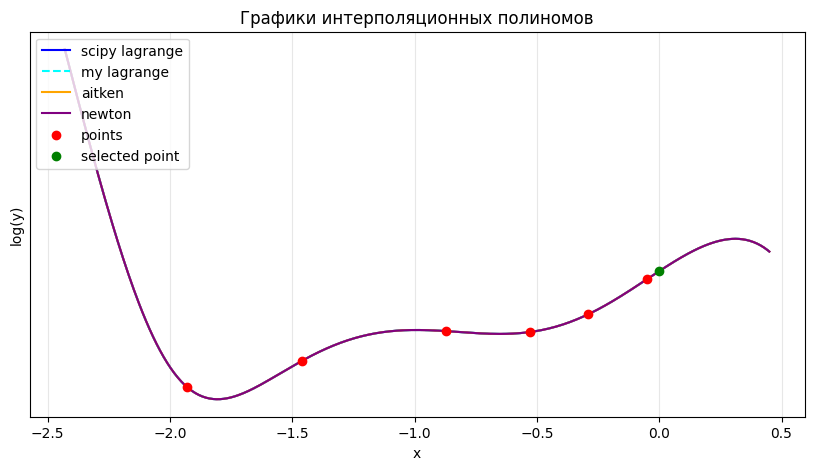
\includegraphics[width=1\textwidth]{pct/plot.png}
    \caption{Сравнение интерполяционных методов (Лагранж, Эйткен, Ньютон) и эталон SciPy; кривые накладываются и видны как единый слой.}
    \label{fig:interp_compare}
\end{figure}

\section{Выводы}
\begin{itemize}
  \item Реализованные методы интерполяции (Лагранж, Эйткен, Ньютон через разделённые разности) эквивалентны по математической конструкции и при корректной реализации для произвольной сетки узлов дают одинаковые значения интерполяционного полинома с точностью до машинной погрешности.
  \item Использование формул с конечными разностями (Стирлинг, Ньютон вперёд/назад) на существенно неравномерной сетке при допущении об "усредненном" шаге приводит к появлению методической погрешности, однако позволяет получить приближённые оценки, если неравномерность сетки мала.
  \item Применение многочлена Стирлинга к точке $x=-0.0$ носит оценочный характер, так как точка находится вблизи правого края таблицы, а не в ее середине, для которой оптимизированы центральные разностные схемы. Также на погрешность повлияло ограничение по учету высоких порядков конечных разностей.
\end{itemize}
